\section{Koncepcia}
Konceptuálny model\cite[str. 13]{ims} vychádza zo získaných dát popísaných v kapitole \ref{sec:rozbor}. Pri tvorení modelu bol kladený dôraz
na vytvorenie výstižného opisu problému a zároveň bol dostatočne abstraktný na to aby zjednodušil simuláciu ale zároveň dostatočne presný na to aby zachytil podstatné aspekty systému. 

\subsection{Spôsob vyjadrenia modelu}
Model je vyjadrený pomocou petriho siete. Zobrazuje prechody medzi jedlotlivými stavmi a čakacie doby. Petriho sieť je možné vidieť na obrázku \ref{fig:petri}.

\begin{figure}[H]
    \centering
    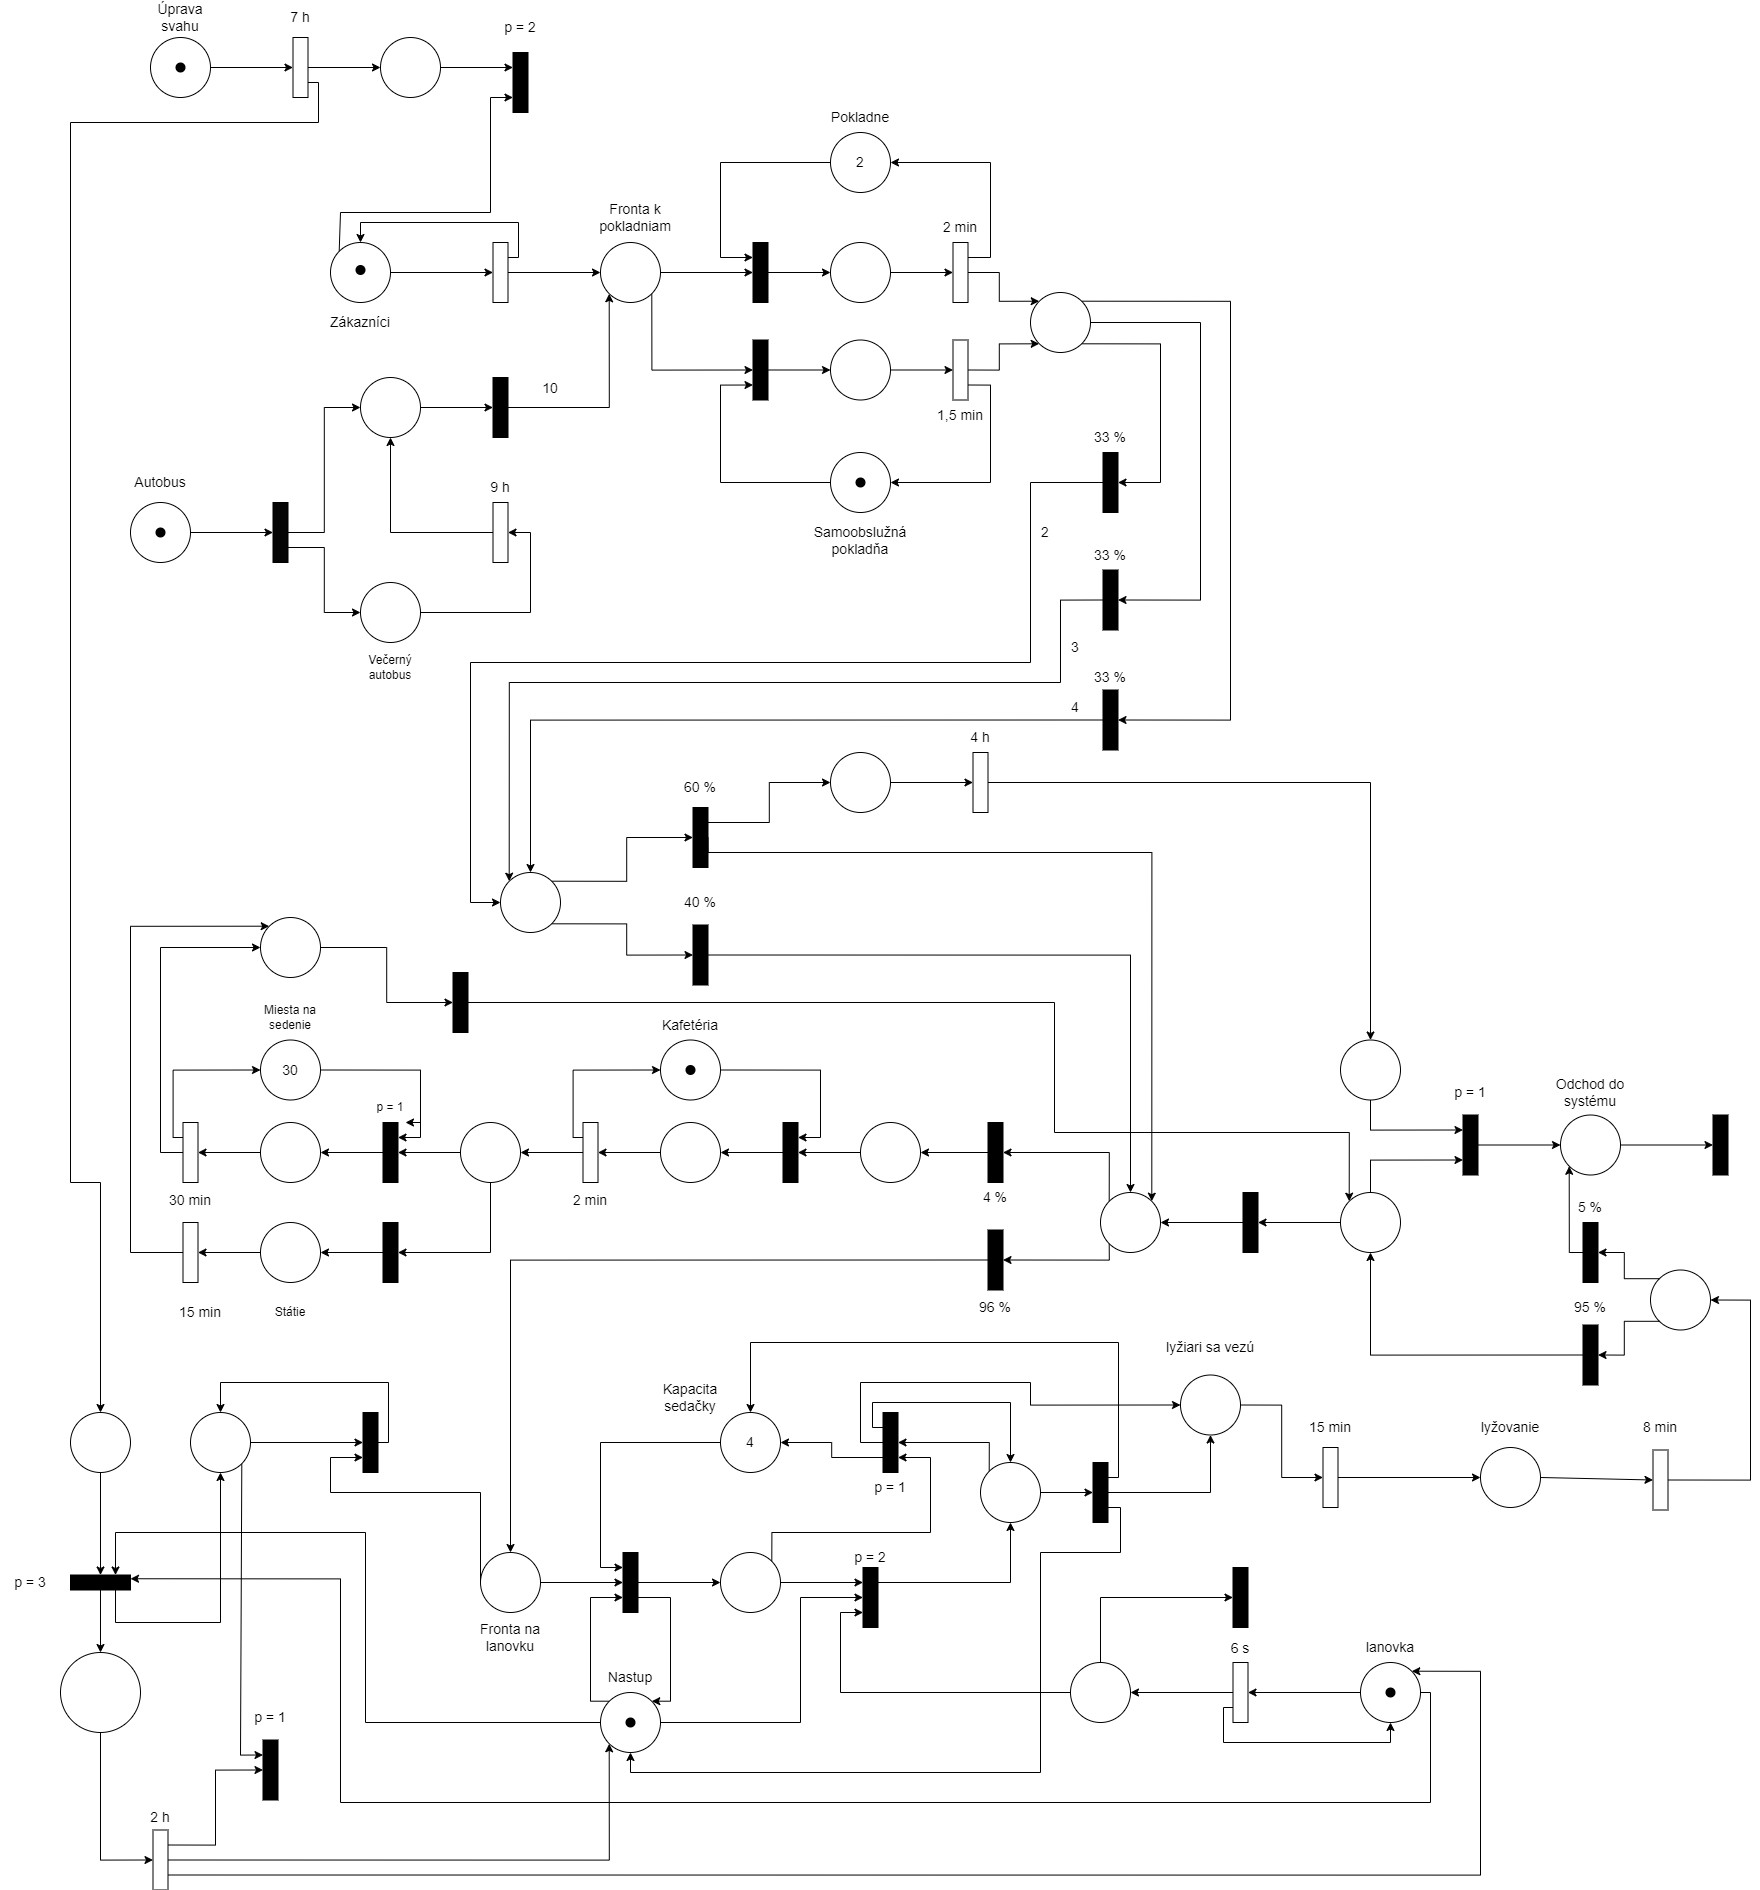
\includegraphics[width=1\textwidth]{petriho-siet.png}
    \caption{Petriho sieť.}
    \label{fig:petri}
  \end{figure}

\subsection{Popis konceptuálneho modelu}
Lyžiarske stredisko Snowparadise Veľká Rača je počas hlavnej sezóny otvorené každý deň od 8:30 do 15:30 pre denné lyžovanie a následne 
od 17:30 do 20:30 pre večerné lyžovanie. O 8:30 prichádza aj prvý skibus s návšetvníkmi, ostatní sa do strediska dopravujú svojpomocne. Po príchode do strediska si musia návšetvníci zakúpiť lístok, toto zariadujú dve obslužné linky. 
Prvá reprezentuje dve pokladne s obsluhou,
v ktorej zakúpenie lístka trvá 2 minúty. Druhá reprezentuje samoobslužný automat, v ktorom zakúpenie lístka trvá 1,5 minúty.
Po zakúpení lístku sa k návšetvníkovi pridá ďaľší 1 až štryria návštevníci, čím bude reprezentovaný reálny priebeh nakupovania lístkov v lyžiaskych strediskách.
(jeden kúpi lístky pre celú rodinu). Následne sú návšetvníci rozdelený v pomere 60 ku 40 do dvoch skupín, pre 4 hodinový lístok a celodenný lístok.
V tomto momente im začína bežať doba lístku. Následne majú na výber ísť na lanovku alebo do kafetérie v pomere 96 ku 4. Sedačky lanovky 
prichádzajú v rozostupoch dlhých 6 sekúnd. Každá sedačka má 4 miesta, vždy berie maximálny možný počet návštevníkov z fronty. Následne
sa návšetvníci vezú 15 minút lanovkou na vrchol kopca. Doba zlyžovania kopca je daná exponenciálnym rozložením s dĺžkou 8 minúty.
Po zlyžovaní majú návštevníci zase možnosť ísť do kafetérie alebo na lanovku. V tomto bode po uplynutí 4 hodinového lístku návšetvník opúšťa stredisko. Taktiež majú možnosť dobrovoľného opustenia strediska s šancou 5\%.
O 15:30 končí denné lyžovanie, lanovka sa vypína a prebieha úprava svahu pre večerné lyžovanie. V tomto čase neprichádzajú noví návštevníci.
Začnú prichádzať o 17:30, zároveň prichádza druhý skibus s návštevníkmi a opätovne sa spúšťa lanovka. 
